Some brief notes before the problems:
\begin{itemize}
    \item \color{brickred}{Koralov and Sinai use $\times$ instead of $\otimes$ for the product $\sigma$-algebra. Moving forward, the reader needs to be cautious about what the operands are. For if they are $\sigma$-algebras, we understand the result of the expression to be the aforementioned product.} 
\end{itemize}
\begin{problem}{1}
\end{problem}
\begin{solution}
    Directly apply the definition of the binomial distribution. Let $X = \{0,1\}$. Define the random variable $\chi_i(\omega)$ for $1\leq i\leq 5$ to be 1 if $\omega = 1$ and zero otherwise. Then, let $\nu_5 = \sum_{i=1}^5 \chi_i$. $\nu_5$ is a binomial random variable. Thus,
    \begin{align*}
        \Pr[\nu_5 = 3] &= \binom{5}{3} \frac{1}{2^5} = \frac{5}{16}.
    \end{align*}
\end{solution}
\begin{problem}{2}
\end{problem}
\begin{solution}
    We present two alternative ways to solve this problem one involving chains and the other geometric series. We first present the solution involving chains. We draw the state space below, where each node denotes a distinct score and the edges between states represent the transition probabilities
    \begin{center}
        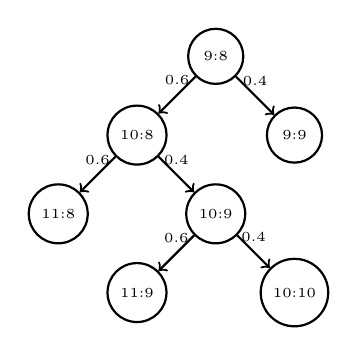
\begin{tikzpicture}[
            n/.style={draw, circle, minimum size=0.7cm, thick},
            p/.style={->, thick}
        ]
            \node[n] (a) at (0,0) {\tiny 9:8};
            \node[n] (b) at (-1,-1) {\tiny 10:8};
            \node[n] (c) at (-2,-2) {\tiny 11:8};
            \node[n] (d) at (0,-2) {\tiny 10:9};
            \node[n] (e) at (-1,-3) {\tiny 11:9};
            \node[n] (f) at (1,-3) {\tiny 10:10};
            \node[n] (g) at (1,-1) {\tiny 9:9};
            \draw[p] (a) -- node[above] {\tiny 0.6} (b);
            \draw[p] (b) -- node[above] {\tiny 0.6} (c);
            \draw[p] (b) -- node[above] {\tiny 0.4} (d);
            \draw[p] (d) -- node[above] {\tiny 0.6} (e);
            \draw[p] (d) -- node[above] {\tiny 0.4} (f);
            \draw[p] (a) -- node[above] {\tiny 0.4} (g);
        \end{tikzpicture}
        \qquad\qquad
        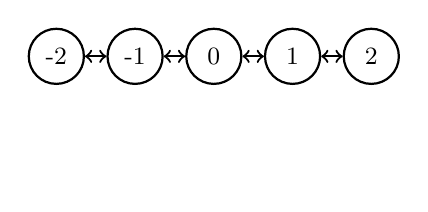
\begin{tikzpicture}[
            n/.style={draw, circle, minimum size=0.7cm, thick},
            p/.style={<->, thick}
        ]
            \node[n] (0) at (0,1.5) {\small 0};
            \node[n] (1) at (1,1.5) {\small 1};
            \node[n] (2) at (2,1.5) {\small 2};
            \node[n] (-1) at (-1,1.5) {\small -1}; 
            \node[n] (-2) at (-2,1.5) {\small -2};
            \draw[p] (0) -- (1);
            \draw[p] (1) -- (2);
            \draw[p] (0) -- (-1);
            \draw[p] (-1) -- (-2);
            \node at (0,0) {};
        \end{tikzpicture}
    \end{center}
    It remains to find the probability that Andrew wins from either 9:9 or 10:10 which is the same since both states require Andrew to win two consecutive points. This, then induces a new chain (see above). Denote by $a,b,c$ the probability that Andrew wins from being one point down, drawn, and one point up. Then, 
    \begin{align*}
        a &= 0.6b, \\
        b &= 0.4a + 0.6c, \\
        c &= 0.4b + 0.6b.
    \end{align*}
    So, $c = 0.36/0.52$. Thus, the probability that Andrew wins is then the aggregate of all states in the chain multiplied by their transition probabilities:
    \[
        \Pr[\text{Andrew wins}] = 0.4\left(\frac{0.36}{0.52}\right) + 0.6\left(0.6 + 0.4\left(0.4\left(\frac{0.36}{0.52}\right) + 0.6\right)\right) = 0.847.  
    \]
\end{solution}
\begin{problem}{3}
\end{problem}
\begin{solution}
    We directly apply the de Moivre-Laplace Theorem. Let $X_i(\omega_i)$ be a random variable that is 1 if $\omega_i =\text{heads}$ and 0 otherwise. Then, let $\nu_n = \sum_{i=1}^n X_i$. Then, for $n=1000$, $\Exp{\nu_n} = 500$ and $\Var{\nu_n} = 250$. $k=600$ as the actual number of heads that we saw during all of the coin flips. Therefore, 
    $z = (600 - 500) / \sqrt{250} = 20/\sqrt(10)$. Therefore, by the de Moivre-Laplace theorem:
    \begin{align*}
        \Pr\left[\frac{\nu_n - \Exp{\nu_n}}{\sqrt{\Var(\nu_n)}} \geq z\right] &\geq \int_{20/\sqrt{10}}^\infty \frac{1}{\sqrt{2\pi}}\exp\left(-\frac{1}{2}z^2\right)~dz, \\
        &\leq 10^{-5}.
    \end{align*}
    So, it is highly unlikely that the coin is fair.
\end{solution}
\begin{problem}{4}
\end{problem}
\begin{solution}
    We show that $\Pr\left[\left|\frac{\nu^n}{n} - p\right| > \epsilon_n\right] \to 0$ as $n\to \infty$:
    \begin{align*}
        \Pr\left[\left|\frac{\nu^n}{n} - p\right| > \epsilon_n\right] &= \Pr[|\nu^n - np| > n\epsilon_n], \\
        &\leq \frac{\Var{\nu^n}}{n^2 \epsilon_n^2}, \\
        &= \frac{np(1-p)}{n(n\epsilon_n)^2}, \\
        &= \frac{p(1-p)}{(\sqrt{n}\epsilon_n)^2} \to 0,
    \end{align*}
    as $n\to\infty$ since $\sqrt{n}\epsilon_n \to \infty$ as $n\to\infty$.

    \textcolor{brickred}{\textit{Remark:}} Even though this problem is fairly simple, it demonstrates something profound about the law of large numbers --- its convergence rate. Specifically, the probability that $\nu^n$ lies in a neighborhood of $O(\sqrt{n})$ tends to 1, as $n\to\infty$. Moreover, the probability that $\nu^n = k$ decays with rate $O(1/\sqrt{n})$ if $k \in (np - O(\sqrt{n}), np + O(\sqrt{n}))$. This is easy to see since we can approximate the distribution within this neighborhood with a crude uniform distribution. Note that this is the exact setup of the De Moivre-Laplace Theorem.
\end{solution}
\begin{problem}{5}
\end{problem}
\begin{solution}
    Let $\nu^n$ be the number of sixes that appear from $n$ tosses of a die. Then, it follows that $\Exp{\nu^{12000}} = 2000$ and $\Var\left[{\nu^{12000}}\right] = 12000\cdot\frac{5}{36} \approx 1666$. Using the de Moivre-Laplace Theorem, we approximate $\frac{\nu^n - \Exp{\nu^n}}{\sqrt{\Var[\nu^n]}}$ as a standard normal distribution. Therefore,
    \[\Pr[1900 \leq \nu^n \leq 2100] = \Phi(2.45) - \Phi(-2.45),\]
    where $\Phi(\cdot)$ is the distribution function of the normal distribution.
\end{solution}
\begin{problem}{6}
\end{problem}
\begin{solution}
    \begin{align*}
        \Pr[\eta_n \leq t] &= 1 - \Pr[\eta_n > t], \\
        &= 1 - \Pr[\omega_i \geq t]^n, \tag{by i.i.d.}, \\
        &= 1 - (1-t)^n.
    \end{align*}
    Next, we evaluate the limit as $n\to\infty$ of $n\eta_n$:
    \begin{align*}
        \lim_{n\to\infty} \Pr[n\eta_n \leq t] &= \lim_{n\to\infty} 1 - \Pr[n\eta_n > t], \\
        &= \lim_{n\to\infty} 1 - \Pr\left[\eta_n > \frac{t}{n}\right], \\
        &= \lim_{n\to\infty} 1 - \left(1 - \frac{t}{n}\right)^n, \\
        &= 1-e^{-t}.
    \end{align*}
\end{solution}
\begin{problem}{7}
    
\end{problem}
\begin{solution}
    
\end{solution}
\begin{problem}{8}
    
\end{problem}
\begin{solution}
    
\end{solution}

\begin{problem}{9}
\end{problem}
\begin{solution}
    
\end{solution}